\documentclass[12pt, fleqn]{article}
\usepackage{../../../template/template}

%сам документ
\begin{document}
\begin{center}
  \huge Практика по геометрии

  (преподаватель Амрани И. М.)

  \large Записал Костин П.А.
\end{center}

Данный документ неидеальный, прошу сообщать о найденных недочетах в \href{https://vk.com/drab_existence_a}{вконтакте}
\tableofcontents
\newpage

\section{Дифференциальная геометрия}
\subsection{(03.09.2019) Кривые и поверхности}
\begin{Example}
    \[\gamma: \R \ra \R^3,\q \gamma \in C^2,\text{ т.ч.}\q |\gamma(t)|=1\ \forall t \in \R\]
    \[\text{Д-ть, что } \gamma'(t) \bot \gamma''(t)\ \forall t \in \R\]
\end{Example}

\begin{Proof}
    \[|\gamma'|=1 \lra \sqrt{<\dot{\gamma},\dot{\gamma}>}=1 \lra <\dot{\gamma},\dot{\gamma}>=1\]
    \[(<\dot{\gamma},\dot{\gamma}>)'=(1)' \Ra 2<\dot{\gamma},\ddot{\gamma}> = 0\]
    Вообще очевидно, но если нет, то:
    \[(<\dot{\gamma},\dot{\gamma}>)'=(\sum_{i=1}^3 \dot{\gamma_i}^2)' = \sum_{i=1}^3 2 \dot{\gamma_i} \ddot{\gamma_i} = 2<\dot{\gamma},\ddot{\gamma}>\]
\end{Proof}

\begin{Example}
    \[\gamma: \R \ra \R^3,\q \gamma \in C^3,\q |\gamma'|=1,\q \gamma'' \neq 0\]
    \[T(t)=\gamma'(t),\q B(t)=T(t) \times N(t),\q N(t)=\frac{\gamma''(t)}{|\gamma''(t)|}\]
    \begin{enumerate}
      \item Д-ть, что $\{T(t), N(t),B(t) \}$ - ОНБ
      \item Найти координаты $\dfrac{dT}{dt}$, $\dfrac{dN}{dt}$, $\dfrac{dB}{dt}$ в базисе $\{T,N,B\}$
    \end{enumerate}
\end{Example}

\begin{sol}
  \begin{enumerate}
    \item Очевидно, $B(t) = \us{=1}{T} \cdot \us{=1}{N} \sin \angle (T,N)$
    \[T \bot N \ (\text{по пред. задаче}),\q B \bot N,\q B \bot T\ (\text{по опр. вект. произв.})\]

    \item По определению "взятием производной"\,получаем:
    \[\dfrac{dT}{dt} = 0T + |\ddot{\gamma}|N + 0B\]
    \[<N, T> = 0 \Ra <\frac{d N}{dt}, T> + <N, \frac{d T}{dt}> = 0\]
    \[\text{Аналогично } 0 = <\frac{d T}{dt},B> = - <\frac{d B}{dt}, T>\]
    \[|\ddot{\gamma}| = <\frac{d N}{dt}, T> = -<N, \frac{d T}{dt}>\]
    \[\frac{d N}{dt} = -|\ddot{\gamma}|T + 0N + \tau(t)B\]
    \[\frac{d B}{dt} = 0T - \tau(t)N + 0B\]
  \end{enumerate}
\end{sol}
\subsection{(10.09.2019) Задачи на кривые}
Мы хотим найти $\tau$ через $\dot{\gamma},\ \ddot{\gamma},\ \dddot{\gamma}$
\begin{remark}
  На плоскоти в каждой точке гладкой кривой есть окружность, которая наилучшим образом приближает кривую
  \[R=\frac{1}{|\ddot{\gamma}|},\q |\ddot{\gamma}| := \ae \text{ - кривизна}\]
  \begin{figure}[h]
	    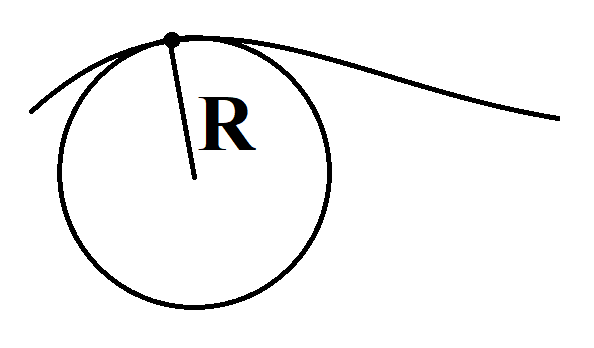
\includegraphics[scale=0.3]{pics/2_1.png}
	    \centering
	\end{figure}
\end{remark}
\begin{Sol} [продолжение]
  \[\tau = <\frac{d N}{dt},\ B>\]
  \[\frac{d N}{dt} = \Br{\frac{\ddot{\gamma}}{\abs{\ddot{\gamma}}}}' = \frac{\dddot{\gamma} |\ddot{\gamma}| - |\ddot{\gamma}|' \ddot{\gamma}}{|\ddot{\gamma}|^2}\]
  \begin{multline*}
    \Ra <\frac{d N}{dt},\ B>=<\frac{\dddot{\gamma} |\ddot{\gamma}| - |\ddot{\gamma}|' \ddot{\gamma}}{|\ddot{\gamma}|^2},\ \frac{\dot{\gamma} \times \ddot{\gamma}}{|\ddot{\gamma}|}> = \\
    \qq \qq = \frac{1}{|\ddot{\gamma}|^3} <\dddot{\gamma} |\ddot{\gamma}|-|\ddot{\gamma}|' \ddot{\gamma},\ \dot{\gamma} \times \ddot{\gamma}> \us{\text{см. на N}}{=} \\
    = \frac{1}{|\ddot{\gamma}|^3} <\dddot{\gamma} |\ddot{\gamma}|,\ \dot{\gamma} \times \ddot{\gamma}> = \frac{1}{|\ddot{\gamma}|^2} <\dddot{\gamma},\ \dot{\gamma} \times \ddot{\gamma} > = \frac{(\dot{\gamma},\ \ddot{\gamma},\ \dddot{\gamma})}{|\ddot{\gamma}|^2}
  \end{multline*}
\end{Sol}

\begin{Example}
  \[\gamma: \R \ra \R^3,\q t \mapsto (4 \cos(t),\ 5-5 \sin(t),\ -3\cos(t))\]
  \begin{enumerate}
    \item Найти $\ae$ и $\tau$
    \item Понять, что из себя представляет линия
  \end{enumerate}
\end{Example}

\begin{sol}
  \begin{enumerate}
    \item Предыдущую задачу мы не можем просто так применить, потому что $|\dot{\gamma}|=5 \neq 1$, но мы можем перепараметризовать:
    \[\w{\gamma}: \R \ra \R^3,\q t \mapsto (4 \cos(\frac{t}{5}),\ 5-5 \sin(\frac{t}{5}),\ -3\cos(\frac{t}{5}))\]
    \[\w{\dot{\gamma}} = (-\frac{4}{5} \sin(\frac{t}{5}),\ -\cos(\frac{t}{5}),\ \frac{3}{5} \sin(\frac{t}{5}))\]
    \[\Ra |\w{\dot{\gamma}}|=1\]
    \[\w{\ddot{\gamma}} = (-\frac{4}{25} \cos(\frac{t}{5}),\ \frac{1}{5} \sin(\frac{t}{5}),\ \frac{3}{25} \cos(\frac{t}{5}))\]
    \[\Ra \ae = |\w{\ddot{\gamma}}| = \frac{1}{25}\]
    \[\w{\dddot{\gamma}} = (\frac{4}{125} \sin(\frac{t}{5}),\ \frac{1}{25} \cos(\frac{t}{5}),\ -\frac{3}{125} \sin(\frac{t}{5}))\]
    \[\Ra \tau = \frac{(\dot{\gamma},\ \ddot{\gamma},\ \dddot{\gamma})}{|\ddot{\gamma}|^2}=25 (\dot{\gamma},\ \ddot{\gamma},\ \dddot{\gamma})=0\]
    \item Наша линия находится на плоскости:
    \[3x+0y+4z\]
    И лежит на сфере:
    \[x^2+(y-5)^2+z^2=25\]
    Значит она представляет из себя окружность, потому что есть разные точки
    \begin{figure}[H]
  	    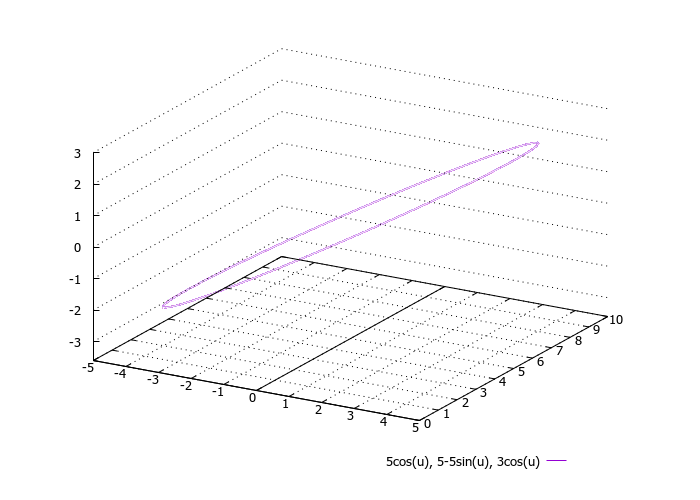
\includegraphics[scale=0.6]{pics/2_2.png}
  	    \centering
  	\end{figure}
  \end{enumerate}
\end{sol}

\begin{Example}
  \[\gamma: \R \ra \R^3,\q t \mapsto (\cos(t),\ \sin(t),\ t)\]
  \begin{enumerate}
    \item Построить график
    \begin{figure}[H]
  	    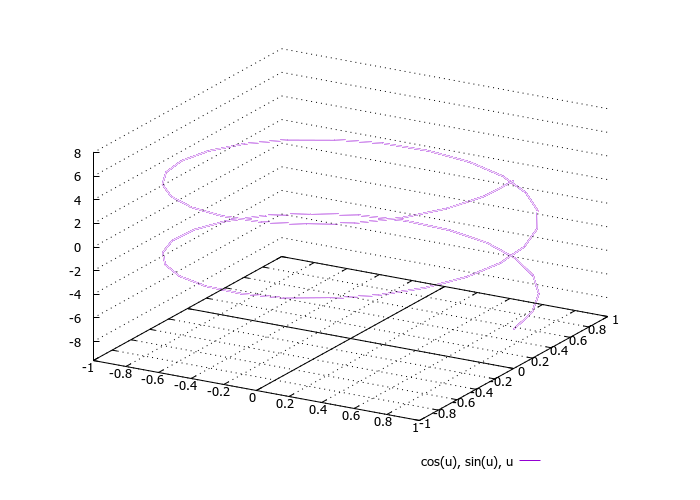
\includegraphics[scale=0.6]{pics/2_3.png}
  	    \centering
  	\end{figure}
    \item Найти $\ae$ и $\tau$
  \end{enumerate}
\end{Example}

\begin{sol}
    Аналогично $t \ra \dfrac{t}{\sqrt{2}}$
    \[\w{\gamma}: \R \ra \R^3,\q t \mapsto (\cos(\frac{t}{\sqrt{2}}),\ \sin(\frac{t}{\sqrt{2}}),\ \frac{t}{\sqrt{2}})\]
    \[\w{\dot{\gamma}}=(-\frac{1}{\sqrt{2}} \sin(\frac{t}{\sqrt{2}}),\ \frac{1}{\sqrt{2}} \cos(\frac{t}{\sqrt{2}}),\ \frac{1}{\sqrt{2}})\]
    \[\Ra |\w{\dot{\gamma}}|=1\]
    \[\w{\ddot{\gamma}}=(-\frac{1}{2} \cos(\frac{t}{\sqrt{2}}),\ -\frac{1}{2} \sin(\frac{t}{\sqrt{2}}),\ 0)\]
    \[\Ra \ae = |\w{\ddot{\gamma}}| = \frac{1}{2}\]
    \[\w{\dddot{\gamma}}=(\frac{1}{2 \sqrt{2}} \sin(\frac{t}{\sqrt{2}}),\ -\frac{1}{2 \sqrt{2}} \cos(\frac{t}{\sqrt{2}}),\ 0)\]
    \[\tau = \frac{(\dot{\gamma},\ \ddot{\gamma},\ \dddot{\gamma})}{|\ddot{\gamma}|^2}\]
    \[(\dot{\gamma},\ \ddot{\gamma},\ \dddot{\gamma}) = \det
    \begin{pmatrix}
      -\frac{1}{\sqrt{2}} \sin(\frac{t}{\sqrt{2}}) & \frac{1}{\sqrt{2}} \cos(\frac{t}{\sqrt{2}}) & \frac{1}{\sqrt{2}}\\
      -\frac{1}{2} \cos(\frac{t}{\sqrt{2}}) & -\frac{1}{2} \sin(\frac{t}{\sqrt{2}}) & 0\\
      \frac{1}{2 \sqrt{2}} \sin(\frac{t}{\sqrt{2}}) & -\frac{1}{2 \sqrt{2}} \cos(\frac{t}{\sqrt{2}}) & 0
    \end{pmatrix} = \frac{1}{8}\]
\end{sol}

\subsection{(17.09.2019) Задачи на поверхности}
\begin{Example}
  \[\gamma: \R \ra \R^3, \q t \mapsto (r(t),\ 0,\ z(t)),\text{ где $r: \R \ra \R$, $z: \R \ra \R$}\]
  Найти параметрищацию поверхности вращения вокруг $OZ$
\end{Example}

\begin{proof}
  Из геометрических соображений: $(r(t) \cos \varphi,\ r(t)\sin \varphi,\ z(t)),\ \varphi \in [0,\ 2\pi]$\\
  Более строго:
  \[\begin{pmatrix}
    \cos \alpha & -\sin \alpha & 0\\
    \sin \alpha & \cos \alpha & 0\\
    0 & 0 & 1
  \end{pmatrix}
  \begin{pmatrix}
    r(t)\\
    0\\
    z(t)
  \end{pmatrix}
  =
  \begin{pmatrix}
    r(t) \cos \alpha\\
    r(t) \sin \alpha\\
    z(t)
  \end{pmatrix}\]
\end{proof}

\begin{definition}
  Гладкая двухмерная поверхность:
  \[F: \os{\text{откр}}{\us{t,\ s}{U}} \subset \R^2 \ra \R^3\]
  т.ч. $\dfrac{\d F}{\d S}$, $\dfrac{\d F}{\d t}$ - непрерывные функции
\end{definition}

\begin{definition}
  Гладкая регулярная поверхность:
  \[F: \os{\text{откр}}{\us{t,\ s}{U}} \subset \R^2 \ra \R^3\]
  т.ч. $\dfrac{\d F}{\d S}$, $\dfrac{\d F}{\d t}$ - линейно независимы\\
  "регулярная = скорость не обнуляется"
\end{definition}
\begin{figure}[H]
    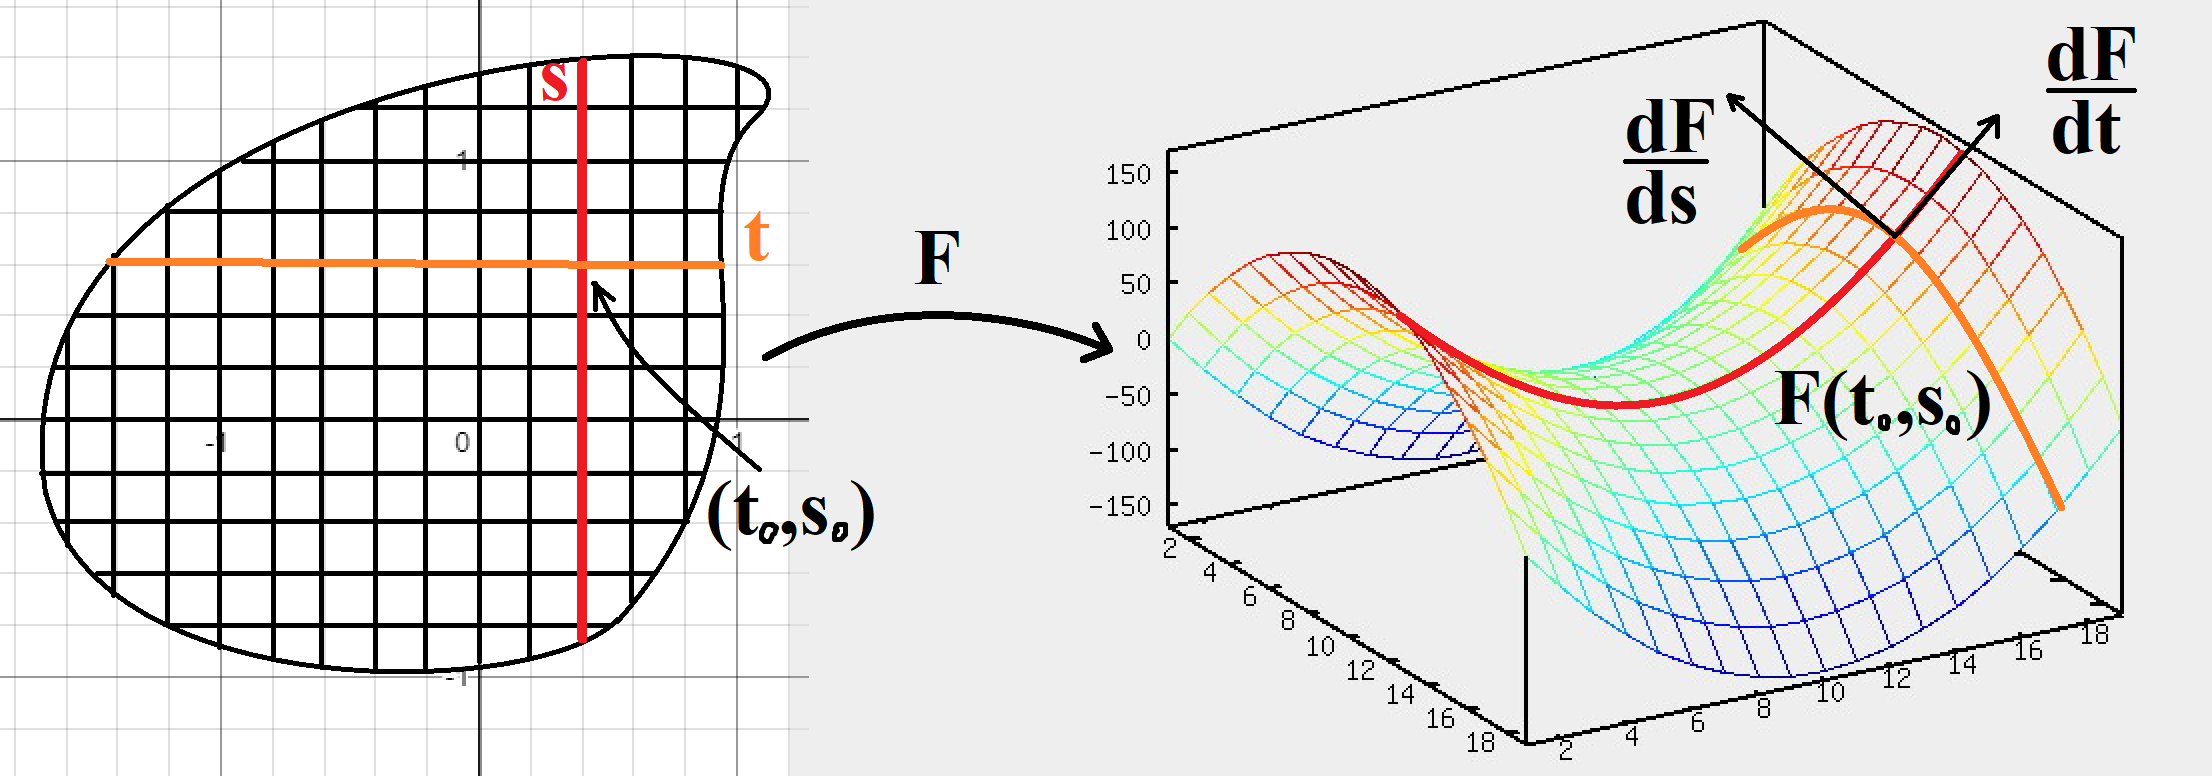
\includegraphics[scale=0.2]{pics/3_1.png}
    \centering
\end{figure}

\subsection{(01.10.2019) Первая и вторая фундаментальные формы }

F

\end{document}
